\documentclass{book}
\usepackage{pgfplots}
\usepackage{imakeidx}
\usepackage{amsfonts}
\usepackage{amsthm}
\usepackage{tikz}
\usepackage{array}
\newcommand{\SectionBreak}{%
    %\vskip 0.5ex

    \nointerlineskip
    \moveright 0.125\textwidth \vbox{\hrule width0.75\textwidth}
    \nointerlineskip
    %\vskip 0.5ex
    \makeatletter
        %\@afterindenfalse%
    \makeatother

}

\newtheorem{definition}{Definizione}

\pgfplotsset{compat=1.18}

\author{F. Piazza \and G. Michieletto}
\title{%
	Appunti di Analisi Matematica II \\
	\large corso della prof.ssa B.Noris \\
	Politecnico di Milano\\
	\bigskip
	\bigskip

	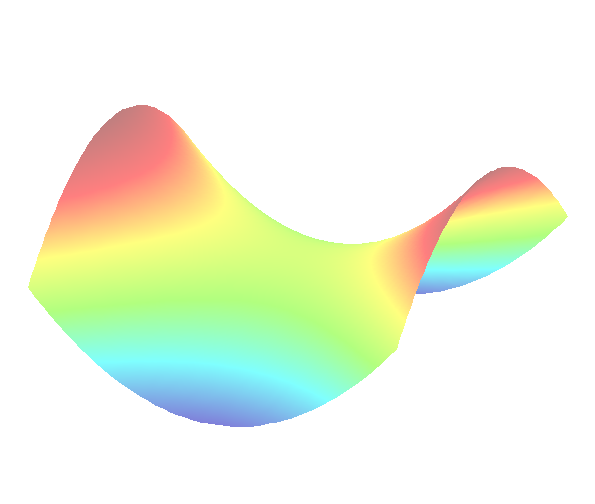
\begin{tikzpicture}
	\begin{axis}[axis line style={draw=none}, colormap/bluered]
	\pgfplotsset{ticks=none}
	\addplot3[surf, samples=50, opacity=0.5, shader=interp] {x^2-y^2};
	\end{axis}
	\end{tikzpicture}
}


\begin{document}


\begin{titlepage}
\maketitle
\end{titlepage}

\chapter{Equazioni differenziali}
\section{Equazioni differenziali del 1° ordine}
\begin{definition}
	Una equazione differenziale o \emph{EDO} del 1° ordine è una relazione tra una funzione $y$ e la sua derivata $y'$ che può essere scritta come
	\begin{equation}
		y' = f(y)
	\end{equation}
	dove $f$ è una funzione continua su un intervallo $I\subseteq\mathbb{R}$.
\end{definition}

Esempi:
\begin{itemize}
	\item $y' = t \sqrt{y_{(t^2)}+1}$ è in forma normale con $f(t,s) = t \sqrt{s^2+1}$. Il dominio di $f$ è $I = \mathbb{R} \times \mathbb{R}$.
	\item $y'_{(t)} = \frac{1}{t}$ con $t>0$ diventa $f(t,s) = \frac{1}{t}$. \textbf{Oss:} $f$ non dipende esplicitamente da $s$. \\ Il dominio di $f$ è $\{(t,s) \in \mathbb{R}^2 : s\in\mathbb{R}, t\in\mathbb{R}^* \}$, dunque è diviso in due parti. Dovrò quindi risolvere la EDO nelle due regioni.
\end{itemize}
\SectionBreak
\begin{definition}
	Si chiama \emph{integrale generale} l'insieme delle soluzioni.
\end{definition}
\begin{definition}
	Si chiama \emph{soluzione particolare} una specifica soluzione.
\end{definition}
\noindent{Una EDO del 1° ordine ha $\infty^1$, soluzioni, cioè avrà una costante arbitraria. In modo analogo, una EDO del 2° ordine avrà $\infty^2$ soluzioni, cioè avrà due costanti arbitrarie.}
Esempi:
\begin{itemize}
	\item integrale generale $ce^t$ con $c$ costante arbitraria. Esempi di soluzioni particolari: $e^t$, $2e^t$, $-e^t$.
	\item $z_{(t)} = -1 + arctan(t)$ con $t\in\mathbb{R}^*$. Esempio di soluzione: $z' = 0 + \frac{1}{1+t^2}$.
\end{itemize}
\textbf{Oss:} La EDO $y'_{(t)} = f(t,y_{(t)})$ è definita per $(t,y)\in dom(f)$

\subsection*{Problema di Cauchy}
\begin{definition}
	Data una EDO del 1° ordine $y'_{(t)} = f(t,y_{(t)})$ sia $(t_{0}, y_{0})$ dove la EDO è definita.
	Cioè $(t_{0},y_{0})\in dom(f)$ \\
	Si chiama \emph{problema di Cauchy} il problema di determinare $y : I\subseteq \mathbb{R} \to \mathbb{R}$ che soddisfa:
	$$ \left\{\begin{array}{lr}y'(t)=f(t,y(t)) \\ y(t_{0})=y_{0}\end{array}\right. $$
\end{definition}
Nota: il sistema ha una condizione perché è del 1° ordine. La condizione trova la soluzione particolare che passa per $(t_{0},y_{0})$.\\
\SectionBreak
\subsection*{Come si risolve?}
Step:
\begin{enumerate}
	\item Trova l'integrale generale. ($\infty^1$ soluzioni dipendenti da 1 parametro)
	\item Impongo la condizione $y(t_{0})=y_{0}$ e la costante $c$
	\item Sostituisco $c$ in 1.
\end{enumerate}

\subsubsection*{Esempi}
Aggiungi Esempi\\
\SectionBreak

\subsection*{EDO 1° ordine lineari}
\begin{definition}
	Una EDO del 1° ordine lineare in forma normale è:\\
	\begin{equation}
		y'_{(t)} = a(t)y_{(t)} + b(t)
	\end{equation}
	dove $a$ e $b$ sono funzioni continue su un intervallo $J$ di $\mathbb{R}$.\\
	\textbf{N.B.} $J$ è il più grande intervallo di $\mathbb{R}$ tale che $a,b\in J$.\\
\end{definition}

\begin{definition}
	Si chiama EDO omogenea associata
	\begin{equation}
		y'_{(t)} = a(t)y_{(t)}\\
	\end{equation}
\end{definition}
Esempio:\\
esempio
\\
\SectionBreak
\subsection*{Principio di sovrapposizione}
prova












\end{document}